%%
%% Automatically generated file from DocOnce source
%% (https://github.com/hplgit/doconce/)
%%

% #define PREAMBLE

% #ifdef PREAMBLE
%-------------------- begin preamble ----------------------

\documentclass[%
oneside,                 % oneside: electronic viewing, twoside: printing
final,                   % draft: marks overfull hboxes, figures with paths
10pt]{article}

\listfiles               %  print all files needed to compile this document

\usepackage{relsize,makeidx,color,setspace,amsmath,amsfonts,amssymb}
\usepackage[table]{xcolor}
\usepackage{bm,ltablex,microtype}

\usepackage[pdftex]{graphicx}

\usepackage[T1]{fontenc}
%\usepackage[latin1]{inputenc}
\usepackage{ucs}
\usepackage[utf8x]{inputenc}

\usepackage{lmodern}         % Latin Modern fonts derived from Computer Modern

% Hyperlinks in PDF:
\definecolor{linkcolor}{rgb}{0,0,0.4}
\usepackage{hyperref}
\hypersetup{
    breaklinks=true,
    colorlinks=true,
    linkcolor=linkcolor,
    urlcolor=linkcolor,
    citecolor=black,
    filecolor=black,
    %filecolor=blue,
    pdfmenubar=true,
    pdftoolbar=true,
    bookmarksdepth=3   % Uncomment (and tweak) for PDF bookmarks with more levels than the TOC
    }
%\hyperbaseurl{}   % hyperlinks are relative to this root

\setcounter{tocdepth}{2}  % levels in table of contents

% Tricks for having figures close to where they are defined:
% 1. define less restrictive rules for where to put figures
\setcounter{topnumber}{2}
\setcounter{bottomnumber}{2}
\setcounter{totalnumber}{4}
\renewcommand{\topfraction}{0.95}
\renewcommand{\bottomfraction}{0.95}
\renewcommand{\textfraction}{0}
\renewcommand{\floatpagefraction}{0.75}
% floatpagefraction must always be less than topfraction!
% 2. ensure all figures are flushed before next section
\usepackage[section]{placeins}
% 3. enable begin{figure}[H] (often leads to ugly pagebreaks)
%\usepackage{float}\restylefloat{figure}

% newcommands for typesetting inline (doconce) comments
\newcommand{\shortinlinecomment}[3]{{\color{red}{\bf #1}: #2}}
\newcommand{\longinlinecomment}[3]{{\color{red}{\bf #1}: #2}}

\usepackage[framemethod=TikZ]{mdframed}

% --- begin definitions of admonition environments ---

% Admonition style "mdfbox" is an oval colored box based on mdframed
% "notice" admon
\definecolor{mdfbox_notice_background}{rgb}{1,1,1}
\newmdenv[
  skipabove=15pt,
  skipbelow=15pt,
  outerlinewidth=0,
  backgroundcolor=mdfbox_notice_background,
  linecolor=black,
  linewidth=2pt,       % frame thickness
  frametitlebackgroundcolor=mdfbox_notice_background,
  frametitlerule=true,
  frametitlefont=\normalfont\bfseries,
  shadow=false,        % frame shadow?
  shadowsize=11pt,
  leftmargin=0,
  rightmargin=0,
  roundcorner=5,
  needspace=0pt,
]{notice_mdfboxmdframed}

\newenvironment{notice_mdfboxadmon}[1][]{
\begin{notice_mdfboxmdframed}[frametitle=#1]
}
{
\end{notice_mdfboxmdframed}
}

% Admonition style "mdfbox" is an oval colored box based on mdframed
% "summary" admon
\definecolor{mdfbox_summary_background}{rgb}{1,1,1}
\newmdenv[
  skipabove=15pt,
  skipbelow=15pt,
  outerlinewidth=0,
  backgroundcolor=mdfbox_summary_background,
  linecolor=black,
  linewidth=2pt,       % frame thickness
  frametitlebackgroundcolor=mdfbox_summary_background,
  frametitlerule=true,
  frametitlefont=\normalfont\bfseries,
  shadow=false,        % frame shadow?
  shadowsize=11pt,
  leftmargin=0,
  rightmargin=0,
  roundcorner=5,
  needspace=0pt,
]{summary_mdfboxmdframed}

\newenvironment{summary_mdfboxadmon}[1][]{
\begin{summary_mdfboxmdframed}[frametitle=#1]
}
{
\end{summary_mdfboxmdframed}
}

% Admonition style "mdfbox" is an oval colored box based on mdframed
% "warning" admon
\definecolor{mdfbox_warning_background}{rgb}{1,1,1}
\newmdenv[
  skipabove=15pt,
  skipbelow=15pt,
  outerlinewidth=0,
  backgroundcolor=mdfbox_warning_background,
  linecolor=black,
  linewidth=2pt,       % frame thickness
  frametitlebackgroundcolor=mdfbox_warning_background,
  frametitlerule=true,
  frametitlefont=\normalfont\bfseries,
  shadow=false,        % frame shadow?
  shadowsize=11pt,
  leftmargin=0,
  rightmargin=0,
  roundcorner=5,
  needspace=0pt,
]{warning_mdfboxmdframed}

\newenvironment{warning_mdfboxadmon}[1][]{
\begin{warning_mdfboxmdframed}[frametitle=#1]
}
{
\end{warning_mdfboxmdframed}
}

% Admonition style "mdfbox" is an oval colored box based on mdframed
% "question" admon
\definecolor{mdfbox_question_background}{rgb}{1,1,1}
\newmdenv[
  skipabove=15pt,
  skipbelow=15pt,
  outerlinewidth=0,
  backgroundcolor=mdfbox_question_background,
  linecolor=black,
  linewidth=2pt,       % frame thickness
  frametitlebackgroundcolor=mdfbox_question_background,
  frametitlerule=true,
  frametitlefont=\normalfont\bfseries,
  shadow=false,        % frame shadow?
  shadowsize=11pt,
  leftmargin=0,
  rightmargin=0,
  roundcorner=5,
  needspace=0pt,
]{question_mdfboxmdframed}

\newenvironment{question_mdfboxadmon}[1][]{
\begin{question_mdfboxmdframed}[frametitle=#1]
}
{
\end{question_mdfboxmdframed}
}

% Admonition style "mdfbox" is an oval colored box based on mdframed
% "block" admon
\definecolor{mdfbox_block_background}{rgb}{1,1,1}
\newmdenv[
  skipabove=15pt,
  skipbelow=15pt,
  outerlinewidth=0,
  backgroundcolor=mdfbox_block_background,
  linecolor=black,
  linewidth=2pt,       % frame thickness
  frametitlebackgroundcolor=mdfbox_block_background,
  frametitlerule=true,
  frametitlefont=\normalfont\bfseries,
  shadow=false,        % frame shadow?
  shadowsize=11pt,
  leftmargin=0,
  rightmargin=0,
  roundcorner=5,
  needspace=0pt,
]{block_mdfboxmdframed}

\newenvironment{block_mdfboxadmon}[1][]{
\begin{block_mdfboxmdframed}[frametitle=#1]
}
{
\end{block_mdfboxmdframed}
}

% --- end of definitions of admonition environments ---

% prevent orhpans and widows
\clubpenalty = 10000
\widowpenalty = 10000

% --- end of standard preamble for documents ---


\usepackage[swedish]{babel}

\raggedbottom
\makeindex
\usepackage[totoc]{idxlayout}   % for index in the toc
\usepackage[nottoc]{tocbibind}  % for references/bibliography in the toc

%-------------------- end preamble ----------------------

\begin{document}

% matching end for #ifdef PREAMBLE
% #endif

\newcommand{\exercisesection}[1]{\subsection*{#1}}

% This file is to be run by preprocess to produce newcommands.tex
% to be included in .tex files.
% There are format-specific tests here for the newcommands (i.e.,
% different definitions of the commands depending on latex or mathjax).

% Newcommands for LaTeX math.
\newcommand{\tp}{\thinspace .}
\renewcommand{\Re}{\bbbr}
\newcommand{\Oof}[1]{\mathcal{O}(#1)}
\newcommand{\Prob}[1]{\hbox{P}(#1)}
\newcommand{\Var}[1]{\hbox{Var}(#1)}
\newcommand{\Cov}[2]{\hbox{Cov}(#1,#2)}
\newcommand{\StDev}[1]{\hbox{StDev}(#1)}

\newcommand{\punkt}{\thinspace .}
\newcommand{\komma}{\thinspace ,}

\newcommand{\vr}{\vec{r}}
\newcommand{\vrp}{\vec{r}\,'}
\newcommand{\erf}{\mathrm{erf}}
\newcommand{\vrho}{\vec{\varrho}}
\newcommand{\vrhop}{\vec{\varrho}\, '}
\newcommand{\sign}{\mathrm{sign}}

\newcommand{\Tr}[1]{\mathrm{Tr}[#1]}
\newcommand{\e}{\varepsilon}
\newcommand{\g}{\gamma}

\newcommand{\half}{\frac{1}{2}}
\newcommand{\vnabla}{\vec{\nabla}}


% Use footnotesize in subscripts
\newcommand{\subsc}[2]{#1_{\mbox{\footnotesize #2}}}




% ------------------- main content ----------------------



% ----------------- title -------------------------

\thispagestyle{empty}

\begin{center}
{\LARGE\bf
\begin{spacing}{1.25}
FFM234, Klassisk fysik och vektorfält - Föreläsningsanteckningar
\end{spacing}
}
\end{center}

% ----------------- author(s) -------------------------

\begin{center}
{\bf \href{{http://fy.chalmers.se/subatom/tsp/}}{Christian Forssén}, Institutionen för fysik, Chalmers, Göteborg, Sverige${}^{}$} \\ [0mm]
\end{center}

\begin{center}
% List of all institutions:
\end{center}
    
% ----------------- end author(s) -------------------------

% --- begin date ---
\begin{center}
Oct 2, 2018
\end{center}
% --- end date ---

\vspace{1cm}


\section*{10. Värmeledning, diffusionsekvation}

Betrakta ett temperaturfält $T(\vec{r},t)$
\begin{itemize}
\item På ett område $V$.

\item Med randvillkor längs $\partial V$.

\item I närvaro av eventuella värmekällor.

\item Med ett explicit tidsberoende.
\end{itemize}

\noindent
Vi söker nu en differentialekvation för detta fält.

\subsection*{Värmeledning (diffusion)}

Vi vet att värme strömmar från varmare till kallare.  Det innebär att
vi har ett flöde av värmeenergi i en riktning som är motsatt $\vnabla T$.


\begin{summary_mdfboxadmon}[Antagande 1]
Värmeströmmen kan skrivas
\begin{equation}
  \vec{q} = -\lambda\vnabla T,
\end{equation}
där $\lambda$ är värmekonduktiviteten (värmeledningsförmågan), och $\vec{q}$ är själva 
värmeflödet med enheten J\,s$^{-1}$\,m$^{-2}$.
\end{summary_mdfboxadmon} % title: Antagande 1




\begin{summary_mdfboxadmon}[Antagande 2]
Värmetätheten $\varepsilon$ är proportionell mot temperaturen
$$
\varepsilon = c \rho T,
$$
där $c$ är värmekapacitiviteten och $\rho$ är densiteten.
\begin{itemize}
\item $[\varepsilon] = \mathrm{J}/\mathrm{m}^3$

\item $[c] = \mathrm{J} \mathrm{kg}^{-1} \mathrm{K}^{-1}$

\item $[\rho] = \mathrm{kg} \mathrm{m}^{-3}$
\end{itemize}

\noindent
\end{summary_mdfboxadmon} % title: Antagande 2



Betrakta nu en volym $V$, vilken begränsas av en sluten yta $S = \partial V$.  
\begin{itemize}
\item Värmeenergin i denna volym är
\end{itemize}

\noindent
\begin{equation}
  H = \int_{V} Tc\rho \mbox{d}V
  \label{eq:H}
\end{equation}
\begin{itemize}
\item Utflödet av värme från denna volym är 
\end{itemize}

\noindent
\begin{equation}
  \oint_{\partial  V} \vec{q}\cdot \mbox{d}\vec{S}.
\end{equation}
Förutsatt att det inte finns några värmekällor i $V$  måste 
utflödet motsvara förändringen per tidsenhet av värmen
i $V$
\begin{equation}
  \frac{\partial H}{\partial t} = - \oint_{\partial  V} {\vec{q}\cdot \mbox{d}S}.
\end{equation}
Med insättning av ekv. (\ref{eq:H}) i VL och användande av Gauss sats i HL fås
\begin{equation}
  \int_{V}
\frac{\partial}{\partial t} \left( Tc\rho \right) \mbox{d}V = -\int_{V} \vnabla \cdot \vec{q}\mbox{d}V.
\label{energi}
\end{equation}
Volymen $V$ är helt godtyckligt vald, så likheten måste gälla för alla volymer $V$. I så fall kan vi sätta integranderna lika med varandra
\begin{equation}
  \frac{\partial}{\partial t}\left(T c\rho\right) = - \vnabla \cdot \vec{q}
= \vnabla \cdot \lambda \vnabla T = \lambda \\Delta T.
\end{equation}

Om vi nu antar att $c$, $\rho$ och $\lambda$  är konstanter, så kan vi skriva ekvationen som
\begin{equation}
  \frac{\partial T}{\partial t} = k \Delta  T,
\end{equation}
där 
\begin{equation}
  k \equiv \frac{\lambda}{c\rho}.
\end{equation}
Den här ekvationen kallas för värmeledningsekvationen. 


\begin{warning_mdfboxadmon}[Kommentar]
Värmeledningsekvationen är en kontinuitetsekvation för värmeenergin. Ni känner antagligen igen härledningen från det liknande bevis som gjordes i kap. 4 i kurskompendiet.
\end{warning_mdfboxadmon} % title: Kommentar



\paragraph{Stationär lösning.}
För en tidsoberoende värmefördelning gäller $\partial T / \partial t = 0$ och därmed
\begin{equation}
  \Delta  T = 0
\end{equation}
som vi kallar för Laplace-ekvation.

\paragraph{Värmekälla.}
Vad händer nu om vi har en värmekälla i volymen $V$?  Antag att värme
produceras av en källa med tätheten $s = s(\vec{r},t)$ med enheten W\,m$^{-3}$.
Då måste vi komplettera ekv. (\ref{energi}) med en term för denna
uppvärmning
\begin{equation}
  \int_{V} \frac{\partial}{\partial t} \left( Tc\rho \right) \mbox{d}V = \int_{V} \lambda 
\Delta  T
\mbox{d}V + \int_{V} s \mbox{d}V.
\end{equation}
Värmeledningsekvationen (med konstant $c,\rho$) blir då
\begin{equation}
  \frac{\partial T}{\partial t} = k \Delta T + \frac{s}{c\rho}.
\end{equation}
\shortinlinecomment{Kommentar 1}{ Vi använder ibland beteckningen $u = s/(c\rho)$, som också kallas för \emph{värmekälltäthet}. }{ Vi använder ibland beteckningen }

Om temperaturfördelningen är tidsoberoende kan vi skriva ekvationen som
\begin{equation}
  \Delta  T = -\frac{s}{\lambda}
\end{equation}
som är ett exempel på Poissons ekvation.
Högerledet kallar vi då för en källterm.


\begin{notice_mdfboxadmon}[Exempel: En-dimensionell värmeledning]

Betrakta ett område $x \in [0,L]$ i en dimension med följande villkor på temperaturfördelningen $T = T(x,t)$
\begin{itemize}
\item Begynnelsevillkor: $T(x,0) = T_0 \sin \frac{\pi x}{L}$.

\item Randvillkor: $T(0,t) = T(L,t) = 0$ (dvs Dirichlets homogena RV).
\end{itemize}

\noindent
\longinlinecomment{Kommentar 2}{ Teckna $T(x,0)$ och jämför gärna med Neumanns homogena randvillkor som hade stoppat värmetransport genom ändarna eftersom $\partial T / \partial x = 0$ (vid $x=0$ och $x=L$). }{ Teckna $T(x,0)$ och jämför }

Finn temperaturfördelningen för $t > 0$ i avsaknad av någon värmekälla.

\paragraph{Lösning:}
Värmeledningsekvationen är
$$
\frac{\partial T(x,t)}{\partial t} - k \frac{\partial^2 T(x,t)}{\partial x^2} = 0.
$$
Notera att 
$$
\frac{\partial^2}{\partial x^2} \sin \frac{\pi x}{L} = - \frac{\pi^2}{L^2} \sin \frac{\pi x}{L},
$$
vilket gör det naturligt att ansätta lösningen $T(x,t) = f(t) \sin \frac{\pi x}{L}$.

Denna ansats uppfyller randvillkoren och begynnelsevillkoret om $f(0) = T_0$. Insättning i värmeledningsekvationen ger
$$
f'(t) \sin \frac{\pi x}{L} + k f(t) \frac{\pi^2}{L^2} \sin \frac{\pi x}{L} = 0,
$$
vilket har lösningen
$$
f(t) = A e^{-\pi^2 k t / L^2},
$$
där $A = T_0$ bestäms av begynnelsevillkoret. Lösningen 
$$
T(x,t) = T_0 e^{-\pi^2 k t / L^2} \sin \frac{\pi x}{L}
$$
innebär att temperaturen minskar kontinuerligt (flödar ut genom ändarna) och att en stationär lösning, $T=0$, erhålls för stora $t$.
\end{notice_mdfboxadmon} % title: Exempel: En-dimensionell värmeledning




\begin{notice_mdfboxadmon}[Exempel: Värmeledning med källterm]

Granitberggrunden i Sverige innehåller en viss mängd
radium, vars radioaktiva sönderfall ger en uppvärming som av en rymdkälla
för värme med konstant källtäthet $\rho_\mathrm{T}$.  Granitens 
värmeledningsförmåga är $\lambda$ (i W\,m$^{-1}$\,K$^{-1}$).  Låt
oss göra det orealistiska antagandet att Jorden alltigenom bestod av granit
med dessa egenskaper.  Hur skulle i så fall den stationära 
temperaturfördelningen i Jordens inre se ut?  Vad blir temperaturen i 
centrum?

\paragraph{Lösning:}
Vi kan ställa upp differentialekvationen
\begin{equation}
  \Delta T = - \frac{\rho_{\rm T}}{\lambda}
\end{equation}
I sfäriska koordinater under antagande om sfärisk symmetri blir ekvationen
\begin{equation}
  \frac{1}{r^2} \frac{\partial}{\partial r}\left(r^2 \frac{\partial T}
{\partial r}\right) = -Q,
\end{equation}
där $Q = \rho_{\rm T}/\lambda$.  Vi kan skriva detta som
\begin{equation}
  \frac{\partial}{\partial r}\left(r^2 \frac{\partial T}
{\partial r}\right) = -Q r^2,
\end{equation}
och sedan integrera en gång.
\begin{equation}
  r^2 \frac{\partial T}{\partial r} = -\frac{1}{3}Qr^3 + A,
\end{equation}
där $A$ är en integrationsvariabel.  Om vi dividerar med $r^2$ får vi
\begin{equation}
  \frac{\partial T}{\partial r} = -\frac{1}{3}Qr + \frac{A}{r^2}.
\end{equation}
Integrerar vi än en gång får vi
\begin{equation}
  T\left(r\right) = - \frac{1}{6} Q r^2 - \frac{A}{r} + B,
\end{equation}
där $B$ är ännu en integrationsvariabel.  Vi måste nu bestämma
värden på de båda integrationsvariablerna.  Först kan vi notera
att det inte finns någon värmepunktkälla, så temperaturen inte bör bli oändlig i Jordens inre, dvs $A = 0$.

För det andra noterar vi att temperaturen vid jordytan, $r = R$, är 
praktiskt taget 0 jämfört med temperaturen i Jordens centrum, så vi
får ekvationen
\begin{equation}
  0 = -\frac{1}{6} Q R^2 + B.
\end{equation}
vilket ger $B = QR^2/6$. Fysikaliskt så är $B$ temperaturen i Jordens centrum.  Om vi sätter in realistiska värden på $\rho_{\rm T} = 5\times
10^{-8}$ W\,m$^{-3}$, $\lambda = 3,5$ W\,m$^{-1}$\,K$^{-1}$ och $R = 6,4\times
10^6$ m, så får vi $B = 6\times 10^5$ K, vilket är en grov
överskattning av den verkliga temperaturen.
\end{notice_mdfboxadmon} % title: Exempel: Värmeledning med källterm



\subsection*{Greensfunktioner för värmeledningsekvationen}

\begin{itemize}
\item Kan vi använda Greensfunktioner för att teckna lösningar till allmänna källfördelningar?

\item Notera att fälten (temperatur, värmekälla) är både rums- och tidsberoende.

\item Ja, det kan man - Greensfunktionen är då lösningen (med givna randvillkor) till värmeledningsekvationen för en punktkälla i både tid och rum.
\end{itemize}

\noindent
\longinlinecomment{Kommentar 3}{ En punktlik energikälla som bara existerar under ett ögonblick, men är precis så stark att den tillförda energimängden är ändlig. Fundera på hur temperaturfältet borde se ut. }{ En punktlik energikälla som }

Vi söker alltså lösningen till Greensfunktionsekvationen svarande mot värmeledningsekvationen:
$$   
\left( \frac{\partial}{\partial t}-k\Delta\right)G(\vec{r},t;\vec{r}{\;}',t')
=\delta^D(\vec{r}-\vec{r}{\;}')\delta(t-t')
$$
på hela $D$-dimensionella rummet $\mathbb{R}^D$. 
Finner vi lösningen till denna ekvation, kan lösningen till värmeledningsekvationen för godtycklig källfördelning $u$ skrivas
$$
T(\vec{r},t)=\int_{-\infty}^\infty dt'\int d^Dx'\, G(\vec{r},t;\vec{r}{\;}',t')u(\vec{r}{\;}',t')
$$
vilket ses genom direkt insättning
\begin{align}
\left( \frac{\partial}{\partial t}-k\Delta\right)T(\vec{r},t)
&=\int_{-\infty}^\infty dt'\int d^Dx'\,
\left( \frac{\partial}{\partial t}-k\Delta\right)G(\vec{r},t;\vec{r}{\;}',t')u(\vec{r}{\;}',t')
\nonumber \\ 
&=\int_{-\infty}^\infty dt'\int d^Dx'\,
\delta^D(\vec{r}-\vec{r}{\;}')\delta(t-t')u(\vec{r}{\;}',t')
=u(\vec{r},t).
\end{align}
som alltså visar att värmeledningsekvationen uppfylls för detta $T$.

\begin{itemize}
\item Vi studerar lösningen på ett oändligt, $D$-dimensionellt rum. 

\item För det första kan vi använda translationsinvarians i rum och tid för att skriva $G(\vec{r},t;\vec{r}{\;}',t') = \tilde G(\vec{r}-\vec{r}{\;}',t-t')$.

\item Följande lösning uppfyller ekvationen
\end{itemize}

\noindent
$$
\tilde G(\vec{r}-\vec{r}\,',t-t')=\frac{\sigma(t-t')}{(4\pi k (t-t'))^{D/2}}
e^{-\frac{|\vec{r}-\vec{r}\,'|^2}{4k(t-t')}},
$$
där $\sigma(t)$ är stegfunktionen som tar värdet $0$ för $t<0$
och $1$ för $t>0$.

Faktorn $\sigma(t-t')$ gör att en källa vid tidpunkten $t'$ bara kan påverka vad som händer vid senare tidpunkter $t\geq t'$, så vi har kausalitet.

Skissa Greensfunktionens utseende för olika $t$:
\begin{itemize}
\item den börjar som en deltafunktion vid $t-t'=0^+$ 

\item för att när tiden går bli bredare och lägre, hela tiden med Gaussisk form. 
\end{itemize}

\noindent
\vspace{6mm}

% inline figure
\centerline{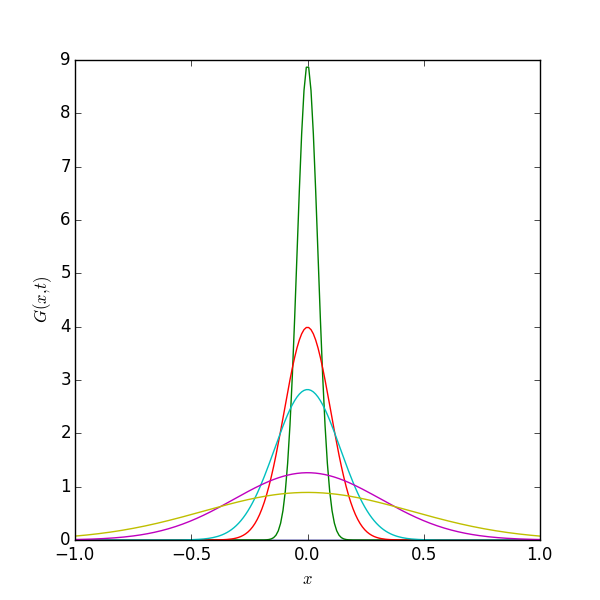
\includegraphics[width=0.95\linewidth]{fig/greens_function_1dim_wtime.png}}

\vspace{6mm}




\begin{warning_mdfboxadmon}[Kommentar]
Det faktum att rumsintegralen av $G$ är konstant i tiden för $t-t'>0$,
$$
\int_{\mathbb{R}^D}d^Dx\,G(\vec{r},\vec{r}\,',t,t')=1,
$$
är ett uttryck för energins bevarande, och naturlig om vi minns att vi kan se värmeledningsekvationen som en kontinuitetsekvation.
\end{warning_mdfboxadmon} % title: Kommentar



Värmeledningsekvationen heter på engelska ``the heat equation''. Dess Greensfunktion kallas ``heat kernel'', på svenska ibland ``värmekärna''.

\subsection*{Värmeledning (konvektion)}

\begin{itemize}
\item Ovan har vi enbart behandlat värmeledning via diffusion.

\item Konvektion erbjuder betydligt effektivare värmetransport för fluider (vätskor och gaser) genom att varm materia strömmar.

\item Vi beskriver detta med en värmeström
\end{itemize}

\noindent
$$
\vec{q}_\mathrm{konv} = \rho c T \vec{v}
$$
som skall adderas till diffusionsströmmen från tidigare
$$
\vec{q}_\mathrm{diff} = - \lambda \vnabla T.
$$
Kontinuitetsekvationen för värmeenergin säger att 
$$
\frac{\partial  T}{\partial t} (T c \rho) = -\vnabla \cdot \vec{q} = -\vnabla \cdot (\vec{q}_\mathrm{diff} + \vec{q}_\mathrm{konv}).
$$
Antar vi återigen att $c$, $\rho$ och $\lambda$ är konstanter (notera att detta innebär att $\vnabla \cdot \vec{v} \propto \partial \rho / \partial t = 0$) får vi
\begin{equation}
  \frac{\partial T}{\partial t} + \vec{v} \cdot \vnabla T = k \Delta  T + \frac{u}{c\rho},
\end{equation}
där vi också inkluderat möjligheten att det finns värmekällor.

% ------------------- end of main content ---------------

% #ifdef PREAMBLE
\end{document}
% #endif

